\section{Methods}
\label{sec:feat_method}

\section{Framework} \label{framework}
Fig. \ref{fig:Framework} illustrates our feature learning and evaluation framework. The individual blocks, such as superpixel segmentation, feature learning methods, and evaluation method, are elaborated in subsequent sections.

\begin{figure}[!htpb]
  \centering
  \includegraphics[width=13cm]{framework/framework}
  \caption[Framework description]{Given a superpixel segmentation and 2D locations, the feature learning algorithm construct a feature matrix $\boldsymbol{X}$, describing each superpixel by a feature. A Random Forest binary classifier is then trained and validated to make predictions of every superpixel. The labels are denoted by $\boldsymbol{y}$, describing if a superpixel belongs to foreground or background. At the bottom-right, we measure the performance of the classifier.}
  \label{fig:Framework}
\end{figure}

Performance evaluation of the different feature learning methods is done on a superpixel level.
In general, superpixelization allows to overcome practical limitations in many applications of computer vision, which may be forbidden due to memory consumption and/or computation time.
This, of course, sometimes bring a significant decrease in the maximal performance of a computer vision task.
We provide quantitative experiments on the latter problem in sec. \ref{sec:superpix}.

Hence, the feature learning methods shall output a feature vector for each of the superpixels. Refer to chapter \ref{superpixel_segm} for more details about the superpixel segmentation.

Let $N$ be the number of images in a data sequence and $S$ the number of superpixels over all sequence. As an example, if we have exactly $200$ superpixels per image, we would have $S=N \cdot 200$ superpixels in that sequence. To every superpixel, we want to assign a feature vector of dimension $D$. We can write the sequence feature matrix as $\boldsymbol{X} = [\boldsymbol{x}_1,...,\boldsymbol{x}_S]^T \in \mathbb{R}^{S \times D}$. Let $\boldsymbol{y} = [y_1,...y_S]^T \in \{0,1\}^S$ be the labels, meaning that $y_i=1$ for superpixels that count to the object of interest and $y_i=0$ for superpixels belonging to the background. Using the feature matrix $\boldsymbol{X}$ and the label vector $\boldsymbol{y}$, a \gls{rf} classifier then calculates performance measures, such as Precision-Recall curve and \textit{max F1-Score}. How the \gls{rf} classifier is applied is described in chapter \ref{random_forest}.

Some feature learning methods will use a user-provided 2D location, if available (see Fig. \ref{fig:Framework}).

We used the superpixel segmentation algorithm ASLIC proposed in \cite{achanta12}.
The original simple linear iterative clustering (SLIC) relies on k-means clustering performed in color the Lab color space and further uses spatial coordinates of pixels.
A trade-off between color similarity and spatial proximity is necessary.
In the SLIC approach, the problem is solved by using a compactness parameter.
For images with both, flat and very textured regions, using the same compactness parameter lead to smooth regular-sized superpixel in the flat regions and highly irregular sized superpixel in textured regions.
The ASLIC approach adaptively chooses the compactness parameter for each superpixel differently.
Fig. \ref{fig:ExSuperpixel} shows an example of using ASLIC on dataset \textit{Slit-Lamp Retina A}.

As parameter, the number of superpixels is crucial. In terms of trade-off, setting a large value will capture the contours of objects more accurately, at the cost of having a higher quantity of samples to predict/classify. We verified that taking $200$ superpixels per frame produces reasonably good segmentation on all our sequences.

Having at disposal ground truth data at pixel-level, we set the values of the output variable $\boldsymbol{y}$ the following way.
If one superpixel is covered by the ground truth pixel-wise segmentation by more than $50\%$ of its area, this specific superpixel is assigned to the foreground. Otherwise, it is assigned to the background.

\section{Feature Learning: Baselines} \label{ch:baselines}
To evaluate the performance of a method, a standard approach is to compare it to baseline methods.
We used three different methods as baselines.
The first method is named \gls{bovw}.
A variant of the \gls{bovw}, \gls{scsp} improves on the latter by bagging words at different spatial resolutions.
Last, we use the features of a Deep Convolutional Network (VGG16) pre-trained for image classification.

\subsection{Bag of Visual Words} \label{bow}
\begingroup
\setlength\intextsep{0pt}
\begin{wrapfigure}[4]{l}[0pt]{1.4cm}

\includegraphics[height=1.5cm]{icons/bovw}
\end{wrapfigure}

\gls{bovw} is an unsupervised feature encoding method successfully utilized in scene classification \cite{zhang15}.
The algorithm can be split into feature learning and feature encoding phase \cite{cheriyadat14}.
Feature learning phase is illustrated in Fig. \ref{fig:subfig:bow_training}.
First, we randomly choose a fixed amount of keypoints over all images in a sequence.
Each keypoint is then described by a SIFT descriptor of dimension 128 \cite{lowe04}.
Subsequently, k-means vector quantization quantizes the keypoint descriptors into $K$ classes \cite{lloyed1982}.
Let $\boldsymbol{F} = [\boldsymbol{f}_1,\cdots,\boldsymbol{f}_M]^T \in \mathbb{R}^{M \times 128}$ the SIFT appearance descriptor of the $M$ keypoints.
Eq. \ref{eq:k_means} describes the k-means objective function, where $\boldsymbol{C} = [\boldsymbol{c}_1,...,\boldsymbol{c}_K]^T \in \mathbb{R}^{K \times 128}$ denotes the codebook.

\begin{equation}
   \min_{\boldsymbol{C}} \sum_{m=1}^M \min_{k=1...K} \|\boldsymbol{f}_m - \boldsymbol{c}_k\|^2
   \label{eq:k_means} 
\end{equation}
\vspace{6pt}

The encoding phase, shown in Fig. \ref{fig:subfig:bow_coding}, consists in describing each pixel by a SIFT descriptor and assigning it to the cluster whose centroids is the closest in terms of Euclidean distance.
The assigned clusters of every pixel in one superpixel are described by a histogram of $K$ bins.
This results in a feature matrix of all superpixels in a sequence being $\boldsymbol{X} = [\boldsymbol{x}_1,\cdots,\boldsymbol{x}_S]^T \in \mathbb{R}^{S \times D}$, where $D = K$.

\begin{figure}[htbp]
  \centering
  \subfloat[BoVW feature learning phase]
  {
    \label{fig:subfig:bow_training}
    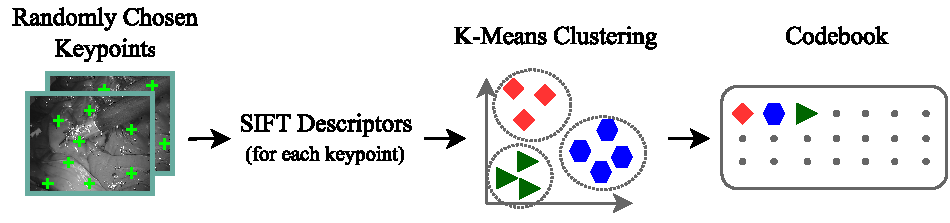
\includegraphics[width=10cm]{bovw/bow_approach_training}
  }
  \\
  \subfloat[BoVW feature encoding phase]
  {
    \label{fig:subfig:bow_coding}
    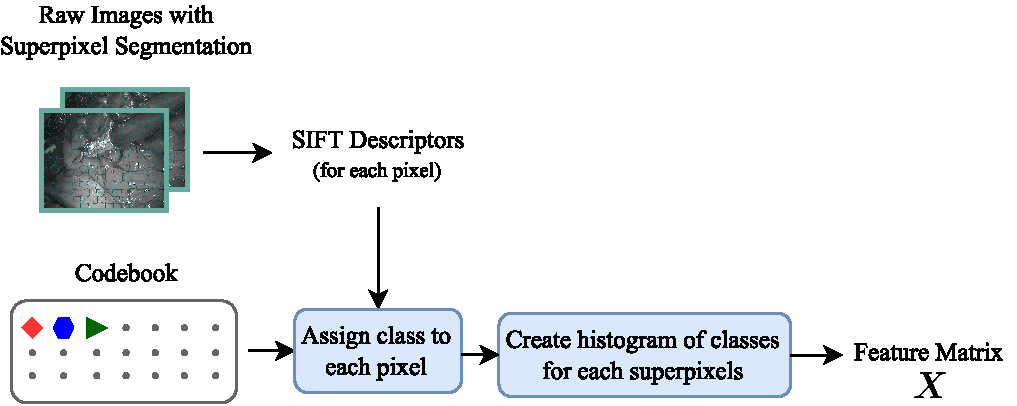
\includegraphics[width=11cm]{bovw/bow_approach_coding}
  }
  \caption[BoVW illustration]{The \gls{bovw} approach is divided in two steps.
    (a) shows the feature learning phase, where SIFT descriptors of randomly chosen keypoints are quantized into a codebook.
    (b) In the encoding phase, each pixel is described by a SIFT descriptor and assigned to a class using the codebook.
    Subsequently, for each superpixel, a histogram of all assigned classes is created, which makes up the final feature descriptor.}
  \label{fig:BoVW_approch}  
\end{figure}

\subsection{Sparse Coded Spatial Pyramid} \label{scp}
\begingroup
\setlength\intextsep{0pt}
\begin{wrapfigure}[4]{l}[0pt]{1.4cm}
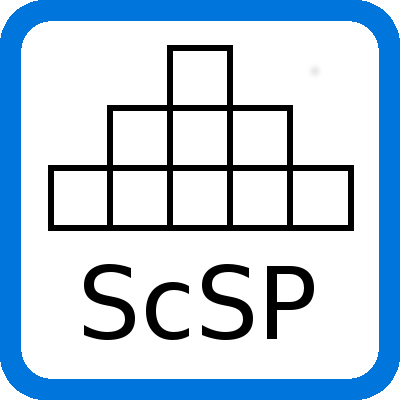
\includegraphics[height=1.5cm]{icons/scsp.png}
\end{wrapfigure}

\gls{scsp} builds up on the \textit{bovw} approach with two main modifications.
A spatial pyramid is a collection of orderless feature histograms computed over cells defined by a multi-level recursive image decomposition \cite{lazebnik09}.

First, instead of the standard k-means clustering, it uses sparse codes of SIFT features.
Second, a pyramid representation is used.
The following describes the added value of \gls{scsp} with \gls{bovw}.

Formally, the objective of sparse coding for vector quantization can be written using matrix computation as shown in Eq. \ref{eq:sparse_codes}.

\begin{equation}
  \min_{\boldsymbol{U,C}} \sum_{m=1}^M \|\boldsymbol{f}_m - \boldsymbol{u}_m \boldsymbol{C}\|^2 + \lambda |\boldsymbol{u}_m|
  \label{eq:sparse_codes} 
\end{equation}
\begin{align*}
  \textrm{subject to } \|\boldsymbol{c}_k\| \leq 1, \hspace{6pt} \forall{k} = 1,2,...,K
\end{align*}

Similar to Eq. \ref{eq:k_means}, $\boldsymbol{f_m}$ represents the SIFT appearance vector of keypoint $m$ and $\boldsymbol{C}$ represents the codebook. $\boldsymbol{U} = [\boldsymbol{u}_1,...,\boldsymbol{u}_M]^T \in \mathbb{R}^{M \times K}$ defines the cluster membership indicator. The L2-norm on $\boldsymbol{c}_k$ is typically applied to avoid trivial solutions. If we drop the regularization term $\lambda |\boldsymbol{u}_m|$ and add a cardinality constraint to $\boldsymbol{u}_m$, meaning that only one element in $\boldsymbol{u}_m$ must be nonzero and positive, the sparse coding formulation in Eq. \ref{eq:sparse_codes} simplifies to k-means objective. Yang et al. \cite{yang09} approved that, compared to standard k-means coding, sparse coding can achieve a much lower reconstruction error due to less restrictive constraints. Sparsity also allows the representation to be specialized and capture salient properties of the image.

Fig. \ref{fig:pyramid_repr} show histograms extracted at different locations on an image.
The final histogram representation is a concatenation of all histograms from all regions.
After normalization, the concatenated histograms can again be seen as a histogram representing the full feature vector.
Hence, for the example shown in Fig. \ref{fig:pyramid_repr} using pyramid levels $\boldsymbol{l} = [1,2,4]$, we have a feature dimension $D = K \cdot (1^2 + 2^2 + 4^2) = K \cdot 21$, where $K$ is the number of classes.

\begin{figure}[htbp]
  \centering
  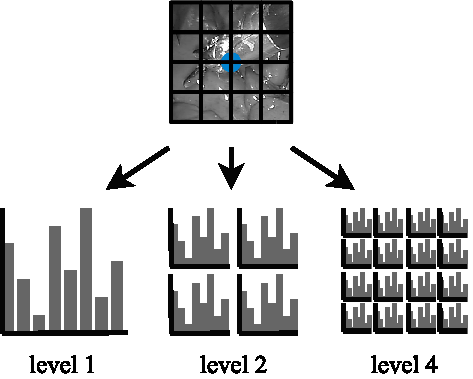
\includegraphics[width=6cm]{scp/pyramid_representation}
  \caption[Spatial pyramid representation]{Illustration of the spatial pyramid representation. Histograms are computed at different levels which are then concatenated into one big vector. After normalization, this vector can again be seen as a histogram vector.}
  \label{fig:pyramid_repr}
\end{figure}

Using a pyramid representation implies that the image patch needs to be square. Intuitively, one wants to enclose within the patch some visual context around the superpixel region. We refer to this parameter as patch size.
In practice, we train our codebook in a similar fashion to \textit{BoVW}, i.e. convert images to grayscale and randomly sample keypoints on every image of the sequence. Each keypoint then gives a SIFT feature vector. Once trained, we extract squared patches of dimension centered on each superpixel's centroid location. We used the implementation of \cite{imdescrip}.

\subsection{Pre-trained VGG-16} \label{vgg}
\begingroup
\setlength\intextsep{0pt}
\begin{wrapfigure}[4]{l}[0pt]{1.4cm}

\includegraphics[height=1.5cm]{icons/vgg.png}
\end{wrapfigure}

VGG is a CNN for large-scale image recognition proposed by \cite{simonyan15}.
The latter work addressed the ImageNet \cite{ILSVRC15} Challenge 2014 (ILSVRC-2014) where it got the first and second places in the localization and classification task, respectively.
Leveraging pre-trained deep networks to address a different task, an approach called transfer learning, has shown its relevance in the frame of semantic segmentation \cite{long15}, emotion recognition \cite{ng15}, and classification \cite{huynh16}.

\endgroup

Here, we use the VGG16 model of \cite{simonyan15}, also known as configuration D \cite[Tab. 1]{simonyan15}.
The model is composed of 16 convolutional layers, each with kernels of size $3 \times 3$.
It is trained for the classification challenge (ImageNet Large Scale Visual Recognition Challenge \cite{ILSVRC15}.
Similar to the \textit{ScSP} approach, we extracted patches at superpixel centroids and fed it to the network.
Since the input dimension of the network is fixed ($244 \times 244 \times 3$), our input data needed to be scaled to that size.
The features are then extracted from the penultimate fully-connected layer, resulting in a feature dimension of $D=4096$.

From a theoretical point of view, let us mention that most machine learning methods make the assumption that training and unseen data lie in the same feature space and have a similar distribution.
However, in many real-world applications, this assumption may not hold \cite{pan2010}.
In a setup where the data distribution of the original training set largely differs from the one we consider, we talk about "Transfer Learning".
We assume that a network pre-trained on a very large-scale dataset with high generalization will produce good features for our task.

\section{Feature Learning: U-Net Based} \label{ch:unet_based}
We now describe our U-Net based feature extraction methods.
We first explain the architecture of the "core" model, i.e. one that will be modified to account for different outputs and loss functions.
We dedicate the second section to data augmentation.
The third section describes how the features can be extracted from the CNN model to obtain feature vectors.
Our various modified U-Nets will then be described in detail.
Finally, an overview summarizes all U-Net based methods.

\subsection{Core Model} \label{model}
Our core model is a slight modification of the original U-Net model \cite{ronneberger15}.
The encoder and decoder are symmetrical units composed of roughly identical blocks.
In particular, each stage, represented as a stack of purple planes on Fig. \ref{fig:unet_model}, is composed of $2$ convolutional layers with $3 \times 3$ kernel size and stride $1$.
The number of filters is increased progressively along with the depth.
A max-pooling operation reduces the size of the feature map by $2$ before passing to the next stage.
Thus, for a depth of $d$ and an input size of $(W, H)$ the spatial resolution at the bottleneck is  $(W /2^d, H/2^{d})$.

This imposes that the input image size must be dividable by $2^{D}$ in order to conserve the same aspect ratio at the output.
Hence, input images were downscaled to the nearest width and height which are dividable by $2^{D}$ before being fed to the network.

We also added batch normalization layers with ReLU activation after each convolutional layers.
Instead of up-convolutional layers in the expansive path (decoder), we used upsampling layers, which apply bi-linear interpolation to increase the resolution.

As shown in \cite{vorontsov17}, this last modification improves prediction performances.
In addition, upsampling layers are parameter-free and allow to reduce the memory requirement.
The last layer of the decoder is a convolutional layer with filter size $1 \times 1$ followed by a sigmoid activation function, which ensures that the output value is between $0$ and $1$.

% In contrast with our baseline approaches, our U-Net methods takes as input the full image instead of patches.
% How the features are then assigned to the individual superpixel is described in chapter \ref{feat_extract}.
% Max pooling downscales the resolution by $2$.
In what follows, we refer to $c\_i$ as the number of input channels and $c\_o$ as the number of output channels.
The input values are scaled to the range $[0,1]$.

\clearpage
\begin{figure}[!htbp]
  \centering
  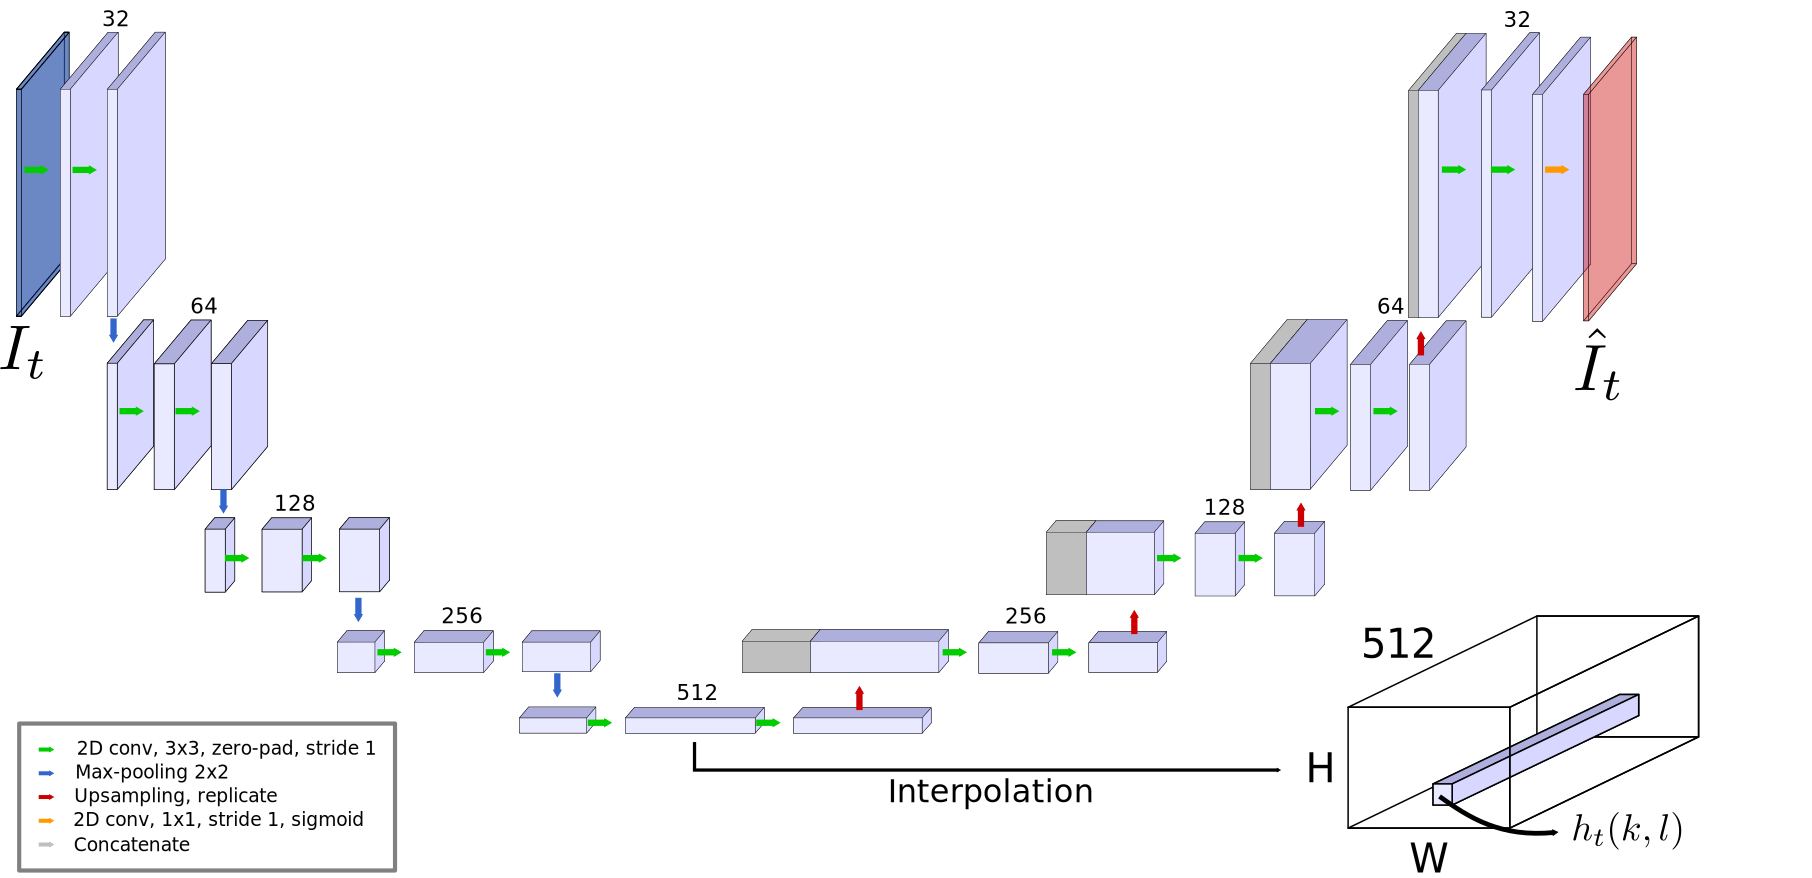
\includegraphics[width=\textwidth]{unet/model}
  \caption[Modified U-Net architecture]{U-Net architecture.
    The number of output channels is indicated above each convolutional layer.
    We add a batch normalization layer after each convolutional layer and remove the skip connections}
  \label{fig:unet_model}
\end{figure}

\subsection{Data Augmentation} \label{ch:data_gen}
As our sequences are limited in size, we resort to data augmentation to artificially increase the training set.
However, since we have a setting where we train the neural network on the same data we later extract the features from, the model does not need to generalize to non-seen data.
Hence, we only consider transformations that correspond to those observed within the original sequence.
For example, it is very likely that during a slit-lamp recording the user rotates and shifts the camera, resulting in different angles and positions of the optical disc.
This confirms to use horizontal and vertical shift, as well as rotation for image transforms.
Contrarily, as the size of the object seldom changes, scaling and zooming are not relevant transformations.
We resort to rotation, vertical/horizontal translation, and shearing.
Additionally, we added Gaussian noise for regularization.
Some examples and parameters used are described in chapter \ref{results_data_gen}.

\clearpage
\subsection{Feature Extraction} \label{feat_extract}
Similarly to our baseline methods, U-Net based methods construct a feature matrix $\boldsymbol{X} = [\boldsymbol{x}_1,...,\boldsymbol{x}_S]^T \in \mathbb{R}^{S \times D}$ describing each superpixel.
Fig. \ref{fig:feat_extract} illustrates this process on an example of a single image.
After training, a forward pass is performed on all image and features are taken as the output (ReLU) of the deepest layer.
Those features correspond to a downscaled version of the input image.
Hence, it must be upscaled to the original image resolution.
Each feature dimension is independently upscaled to the original image size using bicubic interpolation.
Since one pixel becomes a region, extrapolation is also needed at border regions, shown by the red circle and square in Fig. \ref{fig:feat_extract}.
As we now have a descriptor for each pixel upscaled to the same resolution as the original data, we can take the mean over all descriptors belonging to the individual superpixels with feature dimension $D=512$.
\vspace{10pt}

\begin{figure}[htbp]
  \centering
  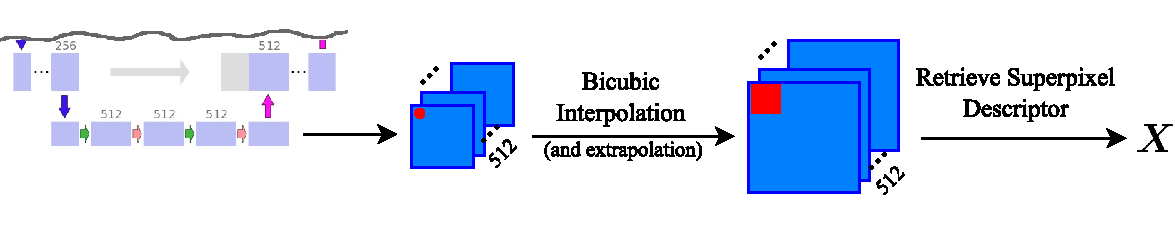
\includegraphics[width=\textwidth]{feat_extract/feature_extraction}
  \caption[Feature extraction model]{Illustration of feature extraction for U-Net based methods.
    The features are extracted from the deepest level.
    Those features are then upsampled on each dimension individually to obtain the input image resolution.
    The feature vector of a given superpixel is taken as the mean of all pixels that it contains.}
  \label{fig:feat_extract}
\end{figure}

\subsection{U-Net Autoencoder}
\begingroup
\setlength\intextsep{0pt}
\begin{wrapfigure}[4]{l}[0pt]{1.4cm}
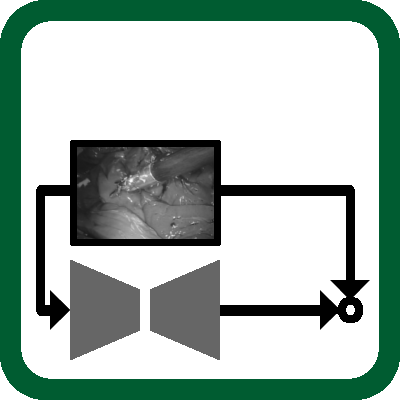
\includegraphics[height=1.5cm]{icons/unet_rec.png}
\end{wrapfigure}

\textit{U-Net Autoencoder} (or \textit{U-Net AE}) is configured as an autoencoder.
It takes as input the image data and reconstructs the same data.
Let $\mathcal{I}$ be the image set and $\boldsymbol{I}_k \in [0,1]^{H \times W \times C}$ an image with height $H$, width $W$ and number of channels $C$.
% We assume that $\boldsymbol{I}_k$ is already downscaled to have $H$ and $W$ dividable by $16$ (see chapter \ref{model}).
Pixels are described by $\boldsymbol{I}_k(i,j,c) \in [0,1]$ with $i$ and $j$ its indices.
The reconstructed image, of same dimension as the input, is written $\boldsymbol{\hat{I}}_k$.
The network's channel dimensions is taken as $C = c_i = c_o$.
We chose to use a mean-squared error (MSE) loss function.
For a minibatch of size $B$, the loss is given by:

\begin{equation}
L_{MSE} = \frac{1}{W H |\mathcal{B}|} \sum_{\boldsymbol{I}_l \in \mathcal{B}} \sum_{i,j,c} \|\boldsymbol{I}_l(i,j,c) - \boldsymbol{\hat{I}}_l(i,j,c)\|^2
\label{eq:mse_loss}
\end{equation}
\vspace{6pt}

Where $\| \cdot \|$ is the $L2$-norm and $\mathcal{B} \subset \mathcal{I}$ is the minibatch.
In later formulations, we will omit the summation on the mini-batch for clarity.

\clearpage
\subsection{U-Net Prior Autoencoder} \label{unet_gaze_rec}
\begingroup
\setlength\intextsep{0pt}
\begin{wrapfigure}[4]{l}[0pt]{1.4cm}
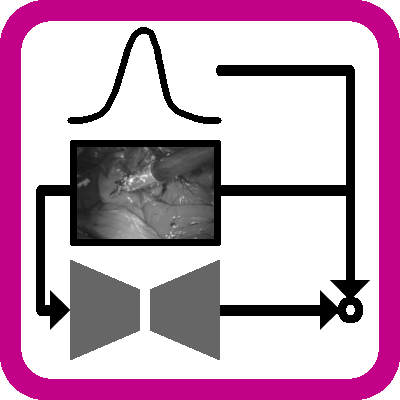
\includegraphics[height=1.5cm]{icons/unet_gaze_rec.png}
\end{wrapfigure}

In contrast with \textit{U-Net Autoenc}, \textit{U-Net Prior AE}, we introduce a prior on the user-provided 2D location in the loss-function.
Let $\boldsymbol{g} = [g_x, g_y]$ be the xy-coordinates of a 2D location, and  $\boldsymbol{Z} \in [0,1]^{H \times W}$ a probability map.
Assuming that $\boldsymbol{g}$ is given for an image $\boldsymbol{I}$, we take $\boldsymbol{Z} \sim \mathcal{N}(\boldsymbol{g}, \sigma^2\mathbb{I})$, a 2D-Gaussian distribution with standard deviation $\sigma$ and mean $\boldsymbol{g}$.
For images where no locations are available, we take a Uniform distribution:
It is formulated in Eq. \ref{eq:gaussian}.

\endgroup

\begin{equation}
\boldsymbol{Z} = 
\begin{cases}
  \mathcal{U}(0,WH),& \textit{if } \boldsymbol{g} \textit{ not available}\\         \mathcal{G}(\boldsymbol{g}, \sigma^2\mathbb{I}),         & \textit{if } \boldsymbol{g} \textit{ available}
\end{cases}
\label{eq:gaussian}
\end{equation}
\hspace{6pt}

$\boldsymbol{Z}_{i,j}$ therefore models the object prior at location $(i,j)$, with $i \in \{\mathbb{Z} \mid 1 \leq i \leq H\}$ and $j \in \{\mathbb{Z} \mid 1 \leq j \leq W\}$ to be the probability of that pixel corresponding to the object of interest. Each pixel's $L2$-norm is then multiplied by $\boldsymbol{Z}_{i,j}$. The loss function is therefore given by:

\begin{equation}
L_{MSE\_Gaze} = \frac{1}{W H} \sum_{i,j} \frac{\boldsymbol{Z}_{i,j}}{\max{\{\boldsymbol{Z}\}}} \|\boldsymbol{I}_{i,j} - \boldsymbol{\hat{I}}_{i,j}\|^2
\label{eq:mse_gaze_loss}
\end{equation}
\hspace{6pt}

Where we normalize by $\max{\{\boldsymbol{Z}\}}$ for later comparison with the loss of \textit{U-Net AE}.
This model, therefore, penalizes errors situated near the 2D locations.
In most image modalities, the object of interest is only a small portion of the image and distinctive.
Contrarily, the background is rather regular or even fully black, as it usually is for CT and MRI scans.
Hence, we speculate that penalizing the loss around the 2D locations equalizes the weights given to background and object of interest in terms of area occupied by the foreground/background, respectively.

\subsection{U-Net Predict Location} \label{sec:unet_pred_loc}

\begin{wrapfigure}[4]{l}[0pt]{1.4cm}
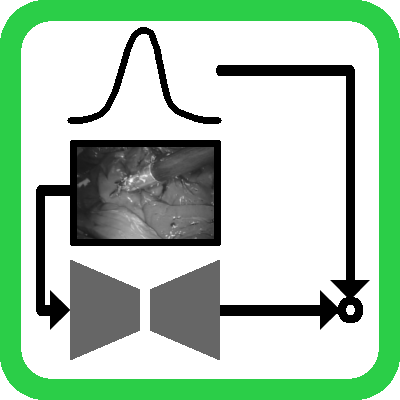
\includegraphics[height=1.5cm]{icons/unet_gaze_prob.png}
\end{wrapfigure}

\textit{U-Net Predict Location} (or \textit{U-Net Pred Loc}) predicts a probability map of the 2D location given the image.
We model the output probability map following eq. \ref{eq:gaussian}.
% The work of \cite{kurmann17}, they used a similar setting and showed that a binary-cross-entropy loss (BCE-loss) performs well.
% This gave rise to use BCE-loss, formulated in Eq. \ref{eq:mse_gaze_prob_loss} on an example of one image. The network's channel dimensions are $c\_i=C$ and $c\_o=1$.
As loss function, we use the cross-entropy loss:

\begin{equation}
L_{BCE} = -\sum_{i,j} \boldsymbol{Z}_{i,j} \log{\boldsymbol{\hat{Z}}_{i,j}}
\label{eq:ce_loss}
\end{equation}
\hspace{6pt}

\clearpage
\subsection{U-Net Predict Location Frozen}

\setlength\intextsep{0pt}
\begin{wrapfigure}[4]{l}[0pt]{1.4cm}
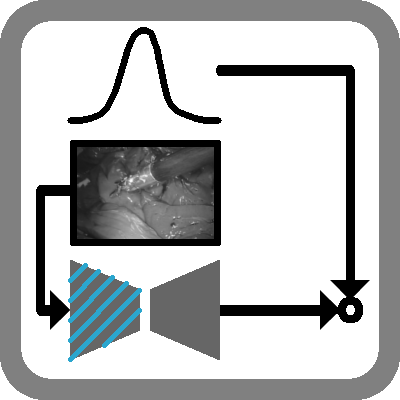
\includegraphics[height=1.5cm]{icons/unet_gaze_prob_freeze.png}
\end{wrapfigure}

\textit{U-Net Predict Location Frozen} (or \textit{U-Net Pred Loc Frozen}) combines the benefits of \textit{U-Net Autoenc} and \textit{U-Net Predict Location}.
The model is first trained as an autoencoder similarly to \textit{U-Net AE}.
Encoder weights are then frozen, and the model is re-trained in a similar fashion to \textit{U-Net Prior Autoenc}.
Fig. \ref{fig:model_freeze} shows the network's portion where weights are frozen.
This method aims at leveraging the benefits of an autoencoder setting while using the location prior as in \textit{U-Net AE}.

\begin{figure}[htbp]
  \centering
  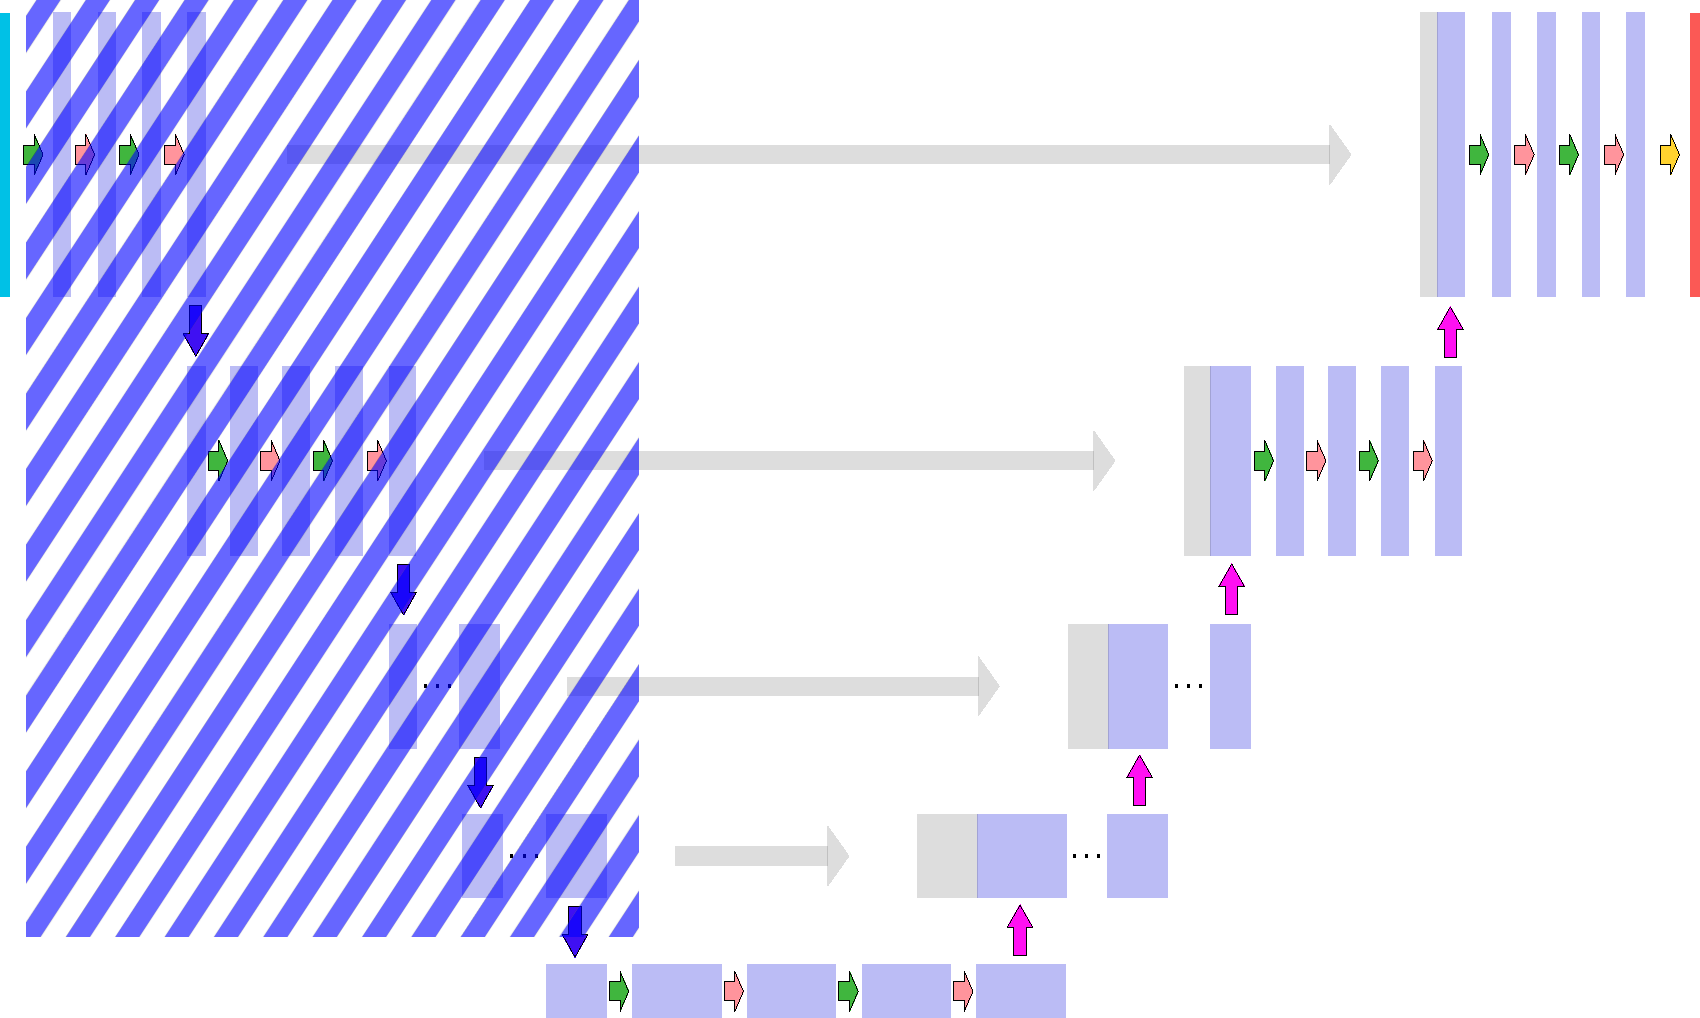
\includegraphics[width=5.0cm]{unet/model5_coarse}
  \caption[Modified U-Net with freezed encoder part]{Illustration of frozen layers in \textit{U-Net Gaze Prob Freeze} method. All encoder part except the lowest level is frozen.}
  \label{fig:model_freeze}
\end{figure}

\subsection{U-Net Motion Predict} \label{sec:unet_pred_loc_concat}
\begingroup
\setlength\intextsep{0pt}
\begin{wrapfigure}[4]{l}[0pt]{1.4cm}
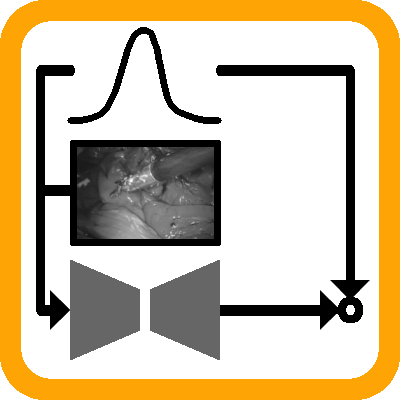
\includegraphics[height=1.5cm]{icons/unet_gaze_prob_concat.png}
\end{wrapfigure}

This model is based on the assumption that objects of interest in our context have relatively slow motion.
In other words, the current user-provided 2D location is correlated to previous 2D locations.
We therefore aim at predicting the object's current location.
\textit{U-Net Motion Predict} (or \textit{U-Net Motion Pred}) incorporates the data's temporal correlation.

Similar to \cite{lea16}, who investigated the problem of fine-grained action segmentation, we increased the model's number of input channel by a motion image.
However, we followed a more straightforward approach by adding as motion information the previous probability map $\boldsymbol{Z}^{(t-1)}$.

Fig. \ref{fig:unet_gaze_concat} illustrates the overall structure on one image $\boldsymbol{I}$.
$\boldsymbol{Z}^{(t-1)}$, the probability map at time $t-1$, is concatenated to $\boldsymbol{I}^{(t)}$.
These are then used to predict the gaze location at time $t$, i.e. $\boldsymbol{\hat{Z}}^{(t)}$.
Similar to \textit{U-Net Predict Location}, we used the \gls{bce} loss function.

\begin{figure}[htbp]
  \centering
  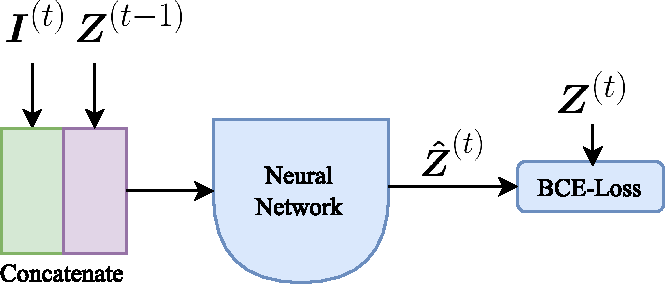
\includegraphics[width=7cm]{unet/unet_gaze_concat}
  \caption[U-Net Motion Predict]{Structure of model \textit{U-Net Motion Predict}.
    The location probability map $\boldsymbol{Z}^{(t-1)}$ is concatenated to the current image data $\boldsymbol{I}^{(t)}$.
    The networks learns to predict the current probability map $\boldsymbol{Z}^{(t)}$.}
  \label{fig:unet_gaze_concat}
\end{figure}

% Since we augmented the inputs by an additional channel, the model's channel dimension become $c\_i=C+1$ and $c\_o=1$.
% Note that in this configuration, the ordering of input frame is substantial. Thus, it made it difficult to apply data augmentation procedure. Due to time limitations, we did not use data augmentation.

\subsection{U-Net Motion Predict LSTM} \label{ch:unet_gaze_prob_lstm}
\begingroup
\setlength\intextsep{0pt}
\begin{wrapfigure}[4]{l}[0pt]{1.4cm}
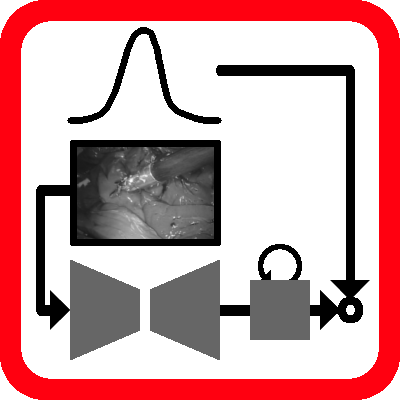
\includegraphics[height=1.5cm]{icons/unet_gaze_prob_lstm}
\end{wrapfigure}

\textit{U-Net Motion Predict LSTM} (or \textit{U-Net Motion Pred LSTM}) also leverages the temporal correlation of the object.
It uses three \textit{U-Net Predict Location} with shared weights to predict three consecutive probability maps.
Those probability maps are fed to a recurrent unit.
In particular, we use a \gls{lstm} \cite{shi15}, to predict the next probability map.
Fig. \ref{fig:unet_gaze_lstm} illustrates this structure.
The \gls{lstm} module uses filters of size $3 \times 3$ and no return sequence.

\endgroup

\begin{figure}[htbp]
  \centering
  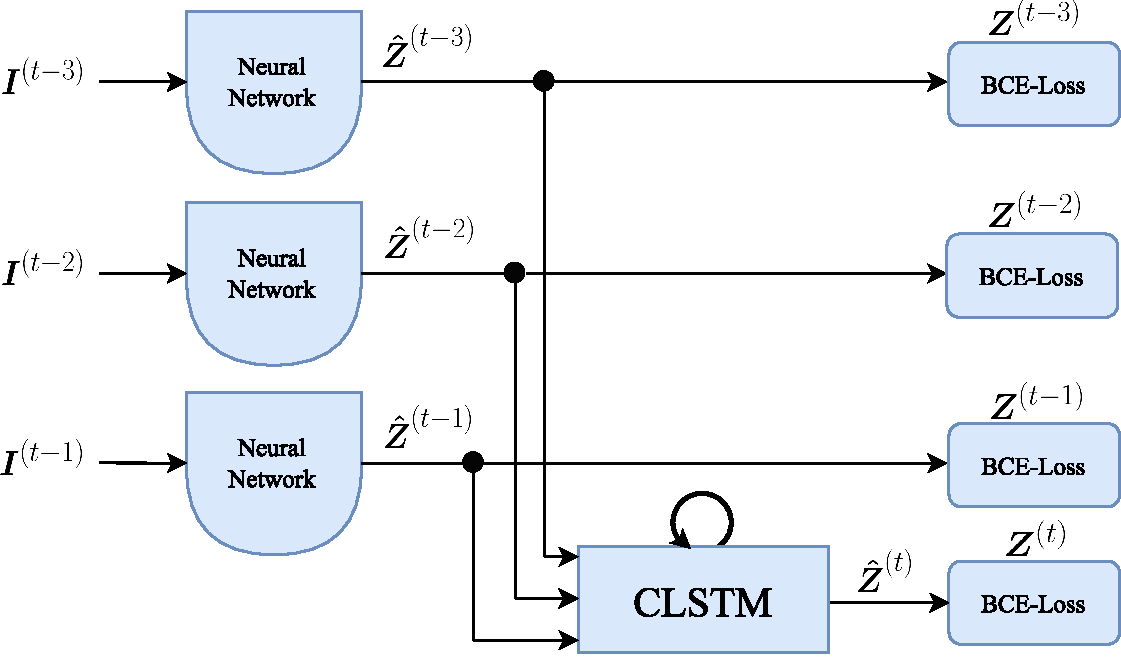
\includegraphics[width=10cm]{unet/unet_gaze_lstm}
  \caption[Structure of U-Net Motion Predict LSTM]{Structure of \textit{U-Net Motion Predict LSTM}.
    A sequence of three images is fed to three identical U-Net models as in \textit{U-Net Pred Location} with shared weights.
    The predicted probability maps $\boldsymbol{\hat{Z}}$ are fed to a \gls{lstm} module to predict the next probability map.}
  \label{fig:unet_gaze_lstm}
\end{figure}

The overall loss $L_{BCE\_LSTM}$ for one image sequence of three images is shown in Eq. \ref{eq:bce_lstm}.
$L_{BCE}(A,B)$ defines the binary cross entropy, formulated in Eq. \ref{eq:mse_gaze_prob_loss}, between $A$ and $B$.
Parameter $\alpha$ is used to adjust the weight of the \gls{lstm} prediction.
We used some jittering to represent the data, i.e. one sample is given by the sequence $[\boldsymbol{I}^{(t=0)}, \boldsymbol{I}^{(t=1)}, \boldsymbol{I}^{(t=2)}]$, and $[\boldsymbol{I}^{(t=1)}, \boldsymbol{I}^{(t=2)}, \boldsymbol{I}^{(t=3)}]$ represents another sample.
% Likewise to the method \textit{U-Net Motion Predict}, we did not synthesize more data by using any sort of data augmentation.

\begin{equation}
L_{BCE\_LSTM} = \alpha \Big[\sum_{d=1}^3 L_{BCE}(\boldsymbol{\hat{Z}}^{(t-d)}, \boldsymbol{Z}^{(t-d)})\Big] + (\alpha - 1) L_{BCE}(\boldsymbol{\hat{Z}}^{(t)}, \boldsymbol{Z}^{(t)})
\label{eq:bce_lstm}
\end{equation}

\subsection{U-Net Based Methods Overview}
Tab. \ref{tab:summary_unet_methods} summarizes the above U-Net based methods.
% To recap, $C$ is the number of image channels ($1$ for grayscale and $3$ for colored) and $c\_i$, $c\_o$ the number of the networks input and output channels, respectively.

\begin{table}[!htbp]
   \centering
   \caption[U-Net based method overview]{Overview of U-Net based methods with $C$ being the number of channels in the images and $c\_i$, $c\_o$ the network's input and output channel dimension, respectively.}
   \begin{tabular}{l|m{1.3cm}|c|c|c|c}
      \toprule
      \textbf{Method} & \textbf{Symbol} & \textbf{Inputs} & \textbf{Labels} & \textbf{c\_i} & \textbf{c\_o} \\
      \midrule
      U-Net Autoencoder & 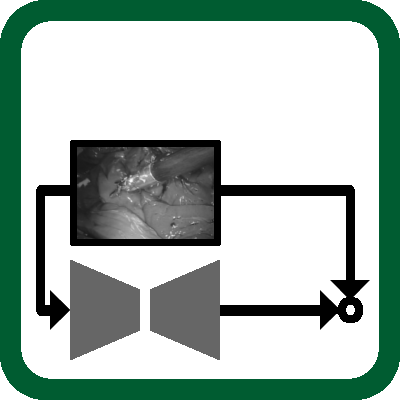
\includegraphics[width=1cm]{icons/unet_rec.png} & Image & Image & $C$ & $C$ \\
      \midrule
      U-Net Prior Autoencoder & 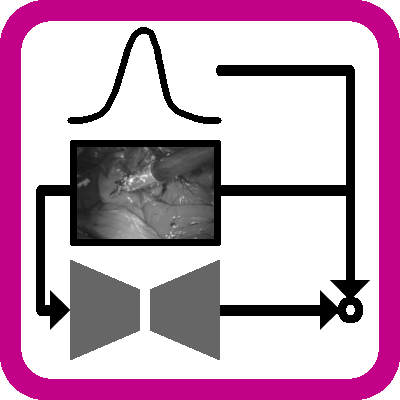
\includegraphics[width=1cm]{icons/unet_gaze_rec.png} & Image & Image \& Gaze & $C$ & $C$ \\
      \midrule
      U-Net Predict Location & 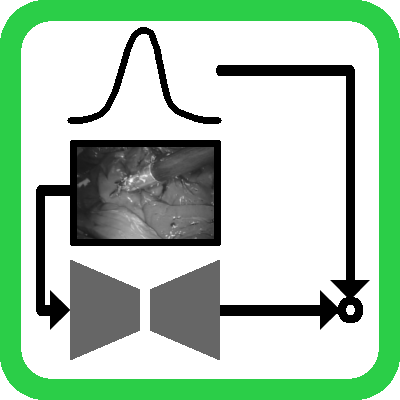
\includegraphics[width=1cm]{icons/unet_gaze_prob.png} & Image & Gaze & $C$ & $1$ \\
      \midrule
      U-Net Predict Location Frozen & 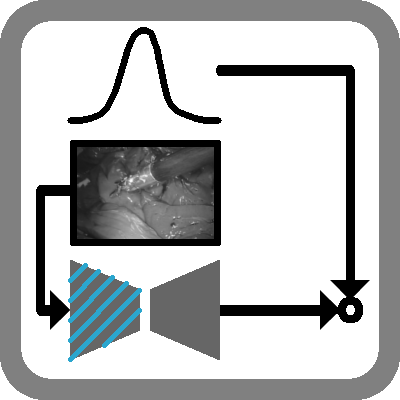
\includegraphics[width=1cm]{icons/unet_gaze_prob_freeze.png} & Image & Gaze & $C$ & $1$ \\
      \midrule
      U-Net Motion Predict & 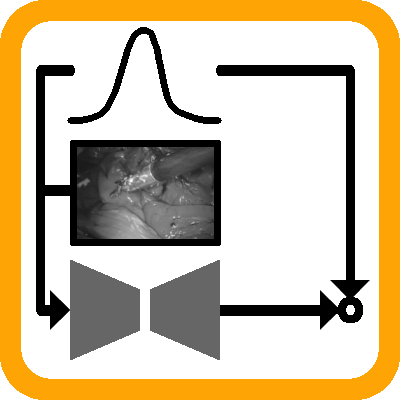
\includegraphics[width=1cm]{icons/unet_gaze_prob_concat.png} & Image \& Gaze & Gaze & $C+1$ & $1$ \\
       \midrule
      U-Net Motion Predict LSTM & 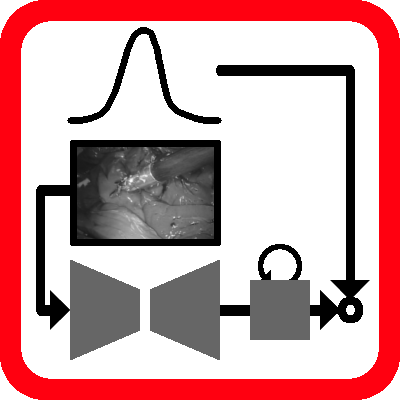
\includegraphics[width=1cm]{icons/unet_gaze_prob_lstm.png} & Image Sequence & Gaze & $3 \times C$ & $3 \times 1$ \\
      \bottomrule
   \end{tabular}
   \label{tab:summary_unet_methods}
\end{table}


\section{Evaluation}
We used a \gls{rf} classifier to compare the performance between the different feature learning methods.
The next section describes further the evaluation phase.


\subsection{Classification} \label{random_forest}
To compare performance between the elaborated methods, we set up a \gls{rf} classifier (Sec. \ref{sec:rf}).
Our pipeline is shown on Fig. \ref{fig:random_forest}.
It takes as input a feature matrix $\bm{X} \in \mathbb{R}^{S \times D}$ and labels $\bm{y} \in \{0,1\}^{S}$ of one image data sequence.
$S$ is the number of superpixels in one sequence and $D$ the feature dimension.
We use 5-fold cross-validation to train the classifier and validate \cite[p. 241]{hastie09}.
Prior to every construction of fold, the samples and their corresponding labels are shuffled.
Each validation set is then evaluated using two metrics: \gls{pr} curve and \textit{max F1-Score}.
The final performance measure is then given by the average performance over all folds.
% Since we usually have very few positive labels, we made in sort that each validation set has approximately the same number of samples.

\begin{figure}[htbp]
  \centering
  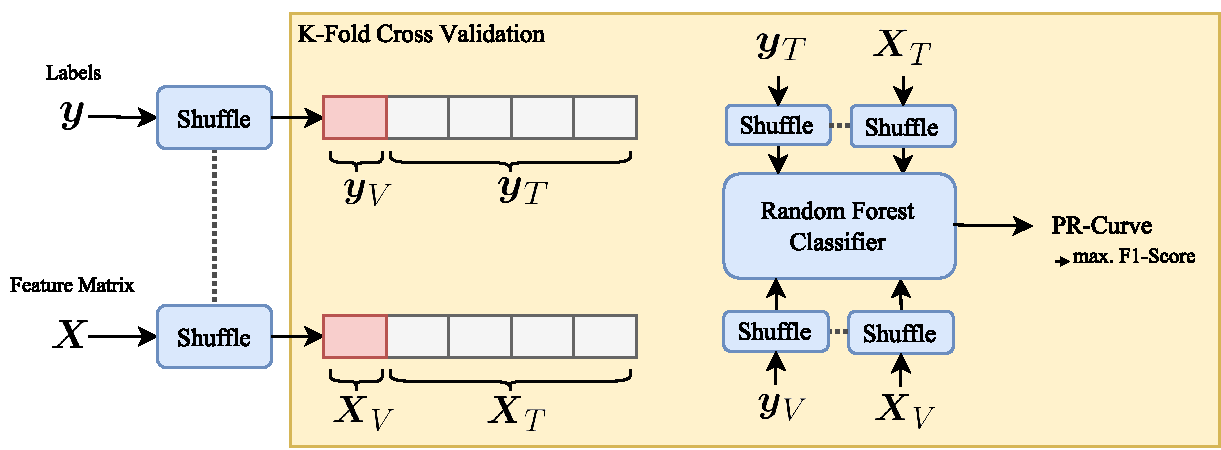
\includegraphics[width=14cm]{random_forest/random_forest}
  \caption[Evaluation pipeline]{Pipeline of the evaluation phase. We fit a \gls{rf} classifier to features $\boldsymbol{X}$, extracted on one sequence, with its corresponding ground truth labels $\boldsymbol{y}$.
    We then perform a k-fold cross-validation.}
  \label{fig:random_forest}
\end{figure}

In our \gls{rf} classifier, all nodes are expanded until the leaves are pure, as advised in \cite[pg. 596]{hastie09}

The forest has $150$ trees and pick $m=\sqrt{D}$ predictor variables, where $D$ is the feature dimension.

\subsection{Performance metrics}
\gls{pr} curves are a performance metric commonly used for binary decision problems in machine learning.
We used PR-curves to evaluate the results of our Random Forest classifier, and thus, PR-curves present the performance of a feature learning method on a dataset.
We also tried using Receiver Operation Characteristics (ROC) as a measure, but it turned out that PR-curves are a more useful measure for our data.
This might be due to the nature of our data.
Since we usually have much more negative than positive labels, our data becomes skewed.
PR-Curves are more informative than ROC for skewed data, as pointed out by \cite{davis06}. They also stated that a curve dominates in ROC space if and only if it dominates in PR space.

F1-Score is a measure that considers both, recall and precision. It's best value is reached at $1$ and worst at $0$. The formula is given by Eq. \ref{eq:f1_score}.

\begin{equation}
\textrm{F1-Score} = 2 \cdot \frac{\textrm{Precision} \cdot \textrm{Recall}}{\textrm{Precision} + \textrm{Recall}}
\label{eq:f1_score}
\end{equation}
\hspace{6pt}

\textit{Max F1-Score} is defined as the relationship between precision and recall that reaches the maximum score. It can be seen as calculating for all points in a PR-curve, their according F1-Scores and taking the maximum. An example is given in Fig. \ref{fig:f1_score}, where the left diagram shows a PR-curve and the right diagram the F1-Score given the Recall values. The maximum value is shown in green.

\begin{figure}[ht]
  \centering
  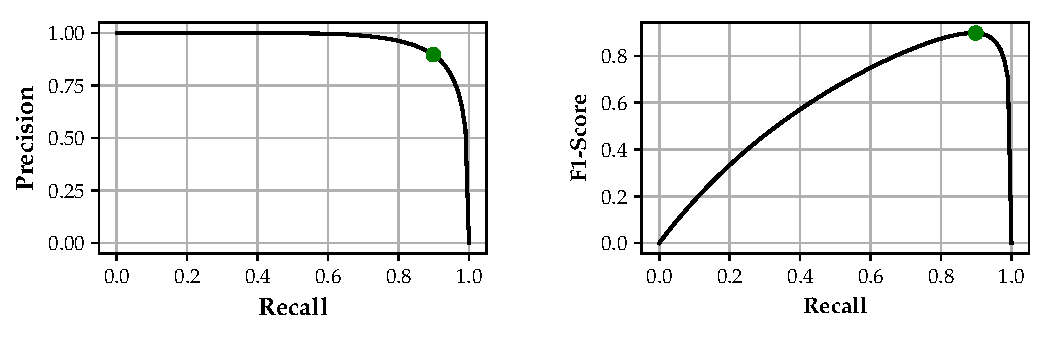
\includegraphics[width=11cm]{f1_score/f1_score}
  \caption[Illustration of max F1-Score]{Illustration of \textit{max F1-Score}. The left diagram shows an example of a \textit{Precision Recall curve}. The diagram on the right shows the F1-Score given the \textit{Recall} values. Maximum score is marked by a green point, the \textit{max F1-Score}.}
  \label{fig:f1_score}
\end{figure}

%%% Local Variables:
%%% mode: latex
%%% TeX-master: "../../main"
%%% End:
